\documentclass{article}
\usepackage{graphicx}
\usepackage{amsmath}
\usepackage{epsf}
\usepackage{xcolor}
\usepackage{float}
% titlepage causes separate title page
% our latex is biased off 1in vertically and horizontally
\newtheorem{theorem}{Theorem}
\setlength{\topmargin}{0.1in}
\setlength{\oddsidemargin}{0in}
\setlength{\evensidemargin}{0in}
\setlength{\headheight}{0in}
\setlength{\headsep}{0in}
\setlength{\textheight}{9in}
\setlength{\textwidth}{6.5in}
% require that floats fill 90% of a page in order for that page to be
% ``float-only''
\renewcommand{\dblfloatpagefraction}{0.9}
\renewcommand{\floatpagefraction}{0.9}
%\renewcommand{\baselinestretch}{1.2} % interline spacing
%\setlength{\parindent}{0in}
%\parskip=10pt plus2pt minus2pt
%\setlength{\unitlength}{0.1in}
%\pagestyle{empty} % no page numbering
\newenvironment{bibparagraph}{\begin{list}{}{ %
    \setlength{\labelsep}{-\leftmargin} %
    \setlength{\labelwidth}{0pt} %
    \setlength{\itemindent}{-\leftmargin} %
    \setlength{\listparindent}{0pt}}}{\end{list}}
\def\makefigure#1#2{\begin{figure}
\begin{center}
\input{#1}
\end{center}
\caption{#2}
\label{#1}
\end{figure}}

\def\limplies{\; \supset \;}
\def\land{\: \wedge \:}
\def\lor{\: \vee \:}
\def\iff{\; \equiv \;}
\def\lnot{\neg}
\def\lforall#1{\forall \: #1 \;}
\def\lexists#1{\exists \: #1 \;}
\def\glitch#1{{\tt #1}} % glitch on
%\def\glitch#1{} % glitch off
\def\comment#1{}
\def\pnil{[\;]}
\def\pif{\; \mbox{\tt :- } \;}
\def\tuple#1{$\langle #1\rangle$}
\def\mtuple#1{\langle #1\rangle}
\def\ceiling#1{\lceil #1\rceil}
\def\floor#1{\lfloor #1\rfloor}
\def\centerps#1{\begin{center}
\leavevmode
\epsfbox{#1}
\end{center}}
\def\argmax{\mathop{\rm argmax}}
\def\argmin{\mathop{\rm argmin}}
\def\grad{\nabla\!}
\def\celsius{^\circ\mbox{C}}
%\long\def\answer#1{}  % comment out for solutions
%\long\def\question#1{#1} % comment out for solutions
\long\def\answer#1{{\color{blue}{\sl #1}}}  % comment in for solution
\long\def\question#1{} % comment in for solution
%\renewcommand{\labelenumi}{(\alph{enumi})}

\def\x{{\bf x}}
\def\w{{\bf w}}

\begin{document}
{\Large
\begin{center}
AI534 --- Written Homework Assignment 3 ---
\end{center}
}
%Please submit electronically via TEACH in a single pdf file.
\begin{enumerate}
\item (Naive Bayes Classifier) (7 pts) Consider the following training set:
\begin{center}
\begin{tabular}{|c|c|c|c|}\hline
A&B&C&Y\\ \hline
0&1&1&0 \\ \hline
1&1&1&0 \\ \hline
0&0&0&0 \\ \hline
1&1&0&1 \\ \hline
0&1&0&1 \\ \hline
1&0&1&1 \\ \hline
\end{tabular}
\end{center}
\begin{enumerate}
\item (3 pts) Learn a Naive Bayes classifier by estimating
all necessary probabilities (there should be 7 independent probabilities to be estimated in total).

\answer{Your answer goes here.
}
\item (3 pts) Compute the probability $P(y=1|A=1, B=0, C=0)$.

\answer{
Your answer goes here.}
\item (1 pts) Suppose we know that the three features A, B and C are independent from one another, can we say that the Naive Bayes assumption is valid? (Note that the particular data set is irrelevant for this question). If your answer is yes, please explain why; if you answer is no please give an counter example.

\answer{Your answer goes here.}

\end{enumerate}

\item (Naive Bayes learns linear decision boundary.) (10 pts) Show that the following naive Bayes classifiers learn linear decision boundary $w_0+w_1x_1+w_2x_2+...+w_dx_d=0$. Express the weights using the corresponding Naive Bayes parameters. Hint: start with the decision boundary defined by $\log\frac{P(y=1|\x)}{P(y=0|\x)}=0$.

\begin{enumerate}
    \item Bernoulli Naive Bayes model, where features $x_1, x_2, ...,x_d$ are binary indicating the presence/absence of words in the vocabulary.\\   
\answer{Your answer goes here.
}
\item Multinomial Naive Bayes Model, where $x_1, ..., x_d$ representing counts of words $w_1, ..., w_d$ in the vocabulary.  Express the weights using the Naive Bayes parameters: the class priors $P(y=1), P(y=0)$ and the class conditionals: $p(w_i|y=1) and p(w_i|y=0)$

\answer{
Your answer goes here.
}
\end{enumerate}

\item (6 pts) Consider the following decision tree:\\
%{\epsfxsize=5in
%\centerps{tree1.eps}
%}
\begin{figure}[h]
\begin{center}
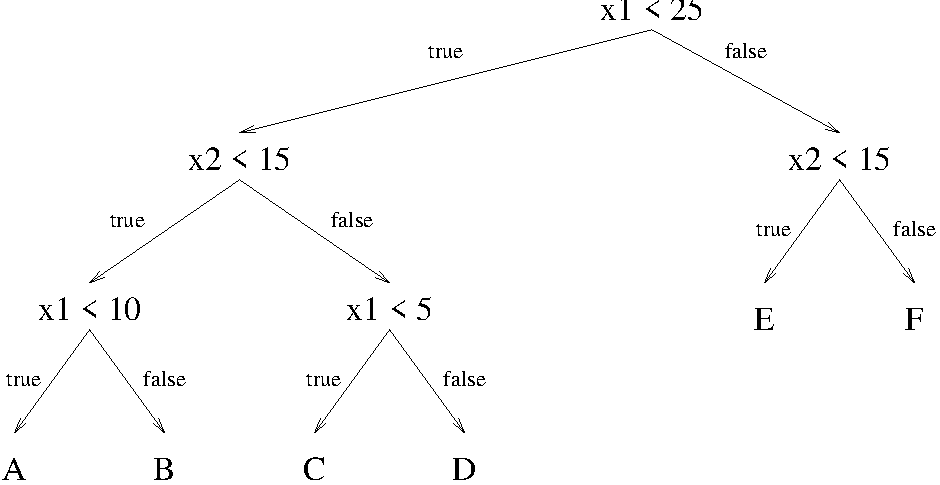
\includegraphics[width=4in]{tree1.pdf}
\end{center}
\end{figure}

\begin{enumerate} 
\item (2 pts) Draw the decision boundaries defined by this tree. Each
leaf of the tree is labeled with a letter.  Write this
letter in the corresponding region of input space.\\

\answer{
Your answer goes here.}

\item (2 pts) Give another decision tree that is syntactically
different but defines the same decision boundaries.  This
demonstrates that the space of decision trees is
syntactically redundant.  \\

\answer{
Your answer goes here.} 

\item (2pts) How does this redundancy influence learning (does it make it easier or harder to find an accurate tree)?

\answer{ your answer goes here.
}

\end{enumerate}
\item (6 pts) In the basic decision tree algorithm (assuming we always create binary splits), we choose the feature/value pair with the maximum information gain as the test to use at each internal node of the decision tree.  Suppose we modified the algorithm to choose at random from among those feature/value combinations that had non-zero mutual information, and we kept all other parts of the algorithm unchanged.

\begin{enumerate}
\item (2 pts) What is the maximum number of leaf nodes that such a
decision tree could contain if it were trained on $m$
training examples?

\answer{Your answer goes here.}

\item (2 pts) What is the maximum number of leaf nodes that a decision
tree could contain if it were trained on $m$ training
examples using the original maximum mutual information
version of the algorithm?  Is it bigger, smaller, or the
same as your answer to (b)?

\answer{Your answer goes here.}

\item (2 pts)How do you think this change (using random splits vs. maximum information mutual information splits) would affect the testing accuracy
of the decision trees produced on average?  Why?

\answer{Your answe goes here.
}

\end{enumerate}
\item (8 pts) Consider the following training set:

\begin{center}
\begin{tabular}{|c|c|c|c|}\hline
A&B&C&Y\\ \hline
0&1&1&0 \\ \hline
1&1&1&0 \\ \hline
0&0&0&0 \\ \hline
1&1&0&1 \\ \hline
0&1&0&1 \\ \hline
1&0&1&1 \\ \hline
\end{tabular}
\end{center}

Learn a decision tree from the training set shown above using the information gain criterion. Show your steps, including the calculation of information gain (you can skip $H(y)$ and just compute $H(y|\x)$) of different candidate tests. You can randomly break ties (or better, choose the one that give you smaller tree if you do a bit look ahead for this problem).

\answer{Your answer goes here.}

\item (8pts) Prove that 
\[ H(X,Y) = H(X)+ H(Y|X) =  H(Y) + H(X|Y)\]. 

Hint: you should start with the definition $H(X,Y) = -\sum_{x,y} P(x,y) \log P(x,y)$. Here we use $X, Y$ to denote the random variables and $x,y$ denote the values $X$ and $Y$ take, $P(x,y)$ is a short hand notation denoting $P(X=x, Y=y)$. 

\answer{
Your answer goes here.}

\end{enumerate}
\end{document}
